%\umlDiagram[box=,sizeX=7cm, sizeY=7cm]{
%	\umlClass[]{Deck}
%	{}
%	{
%		\umlMethod[visibility]{add}{c \emph{BasicCard}}
%		\umlMethod[visibility]{remove}{c \emph{BasicCard}}
%		\umlMethod[visibility]{remove}{i \emph{int}}
%	}
%}
\begin{figure}[h]
	\centering
	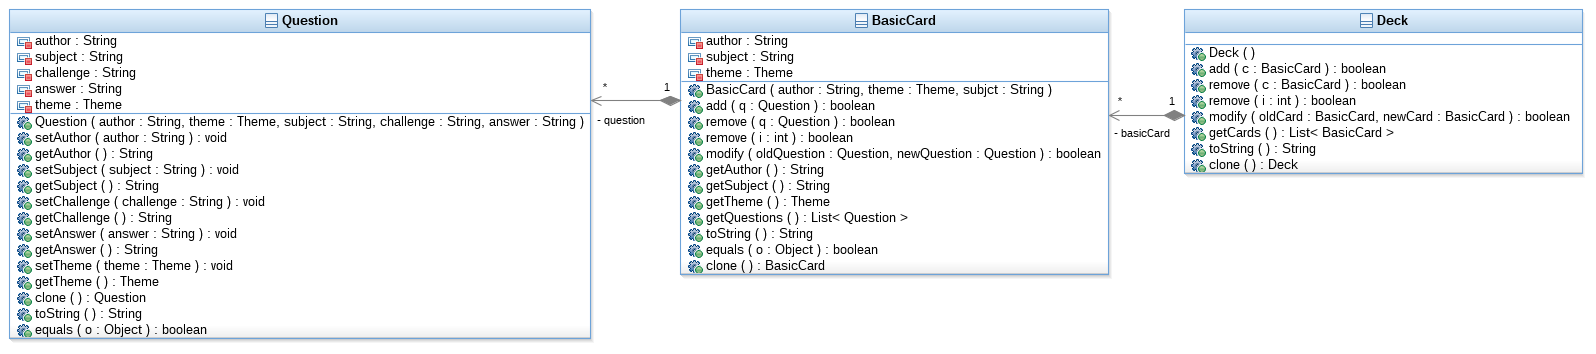
\includegraphics[width=\textwidth]{ttmc_modele.png}
	\caption{Diagramme de classe du modèle}
	\label{fig:diag_modele}
\end{figure}

\begin{figure}[h]
	\centering
	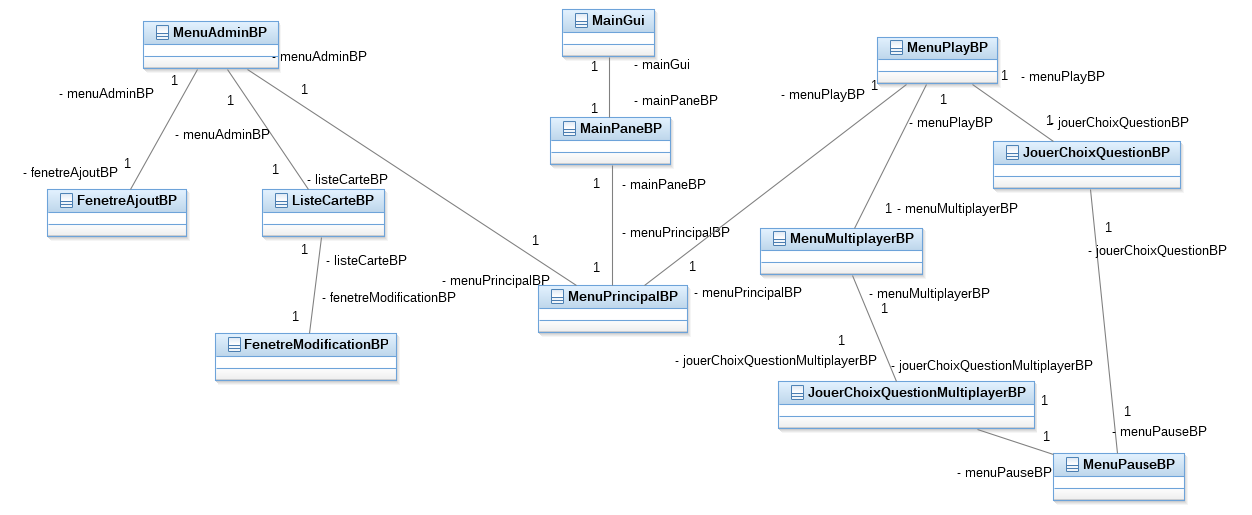
\includegraphics[width=\textwidth]{ttmc_vue.png}
	\caption{Diagramme de classe de la vue}
	\label{fig:diag_vue}
\end{figure}

Nous avons décidé de travailler avec le MainGui en position principale.
Lorsque nous changeons de menu via le click d’un bouton, nous modifions la scène via différents StackPane inclus dans les différentes classes.
Ce qui nous permet d’avoir une répartition plus flexible des menus ainsi qu'une plus grande liberté lors des instantiations de ceux-ci.
Grâce aux StackPanes, on a su faire plusieurs réinstantiations d'un même menu, ce qui nous a permis de démarrer des nouvelles parties à chaque instance d'une partie solo ou multi joueur.
